\documentclass{standalone}
\usepackage{tikz}

\begin{document}
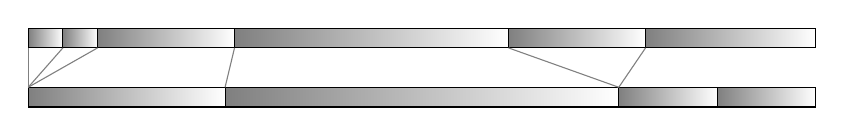
\begin{tikzpicture}

% \draw[help lines, color=gray!30] (-1,2) grid (11,-2);

\tikzstyle{every path}=[draw] % all paths are drawn
% \fill (0,0) rectangle +(1,1);
\shade [shading=axis,shading angle=90](0,0) rectangle +(0.44,.25);
\shade [shading=axis,shading angle=90](0.44,0) rectangle +(0.44,.25);
\shade [shading=axis,shading angle=90](0.88,0) rectangle +(1.74,.25);
\shade [shading=axis,shading angle=90](2.62,0) rectangle +(3.48,.25);
\shade [shading=axis,shading angle=90](6.1,0) rectangle +(1.74,.25);
\shade [shading=axis,shading angle=90](7.84,0) rectangle +(2.16,.25);

% Quant = 2
\shade [shading=axis,shading angle=90](0,-.75) rectangle +(2.5,.25);
\shade [shading=axis,shading angle=90](2.5,-.75) rectangle +(5,.25);
\shade [shading=axis,shading angle=90](7.5,-.75) rectangle +(1.25,.25);
\shade [shading=axis,shading angle=90](8.75,-.75) rectangle +(1.25,.25);
\draw[gray] (0,0) -- (0,-.5);
\draw[gray] (0.44,0) -- (0,-.5);
\draw[gray] (0.88,0) -- (0,-.5);
\draw[gray] (2.62,0) -- (2.5,-.5);
\draw[gray] (6.1,0) -- (7.5,-.5);
\draw[gray] (7.84,0) -- (7.5,-.5);



% Quant = 0
%\shade [shading=axis,shading angle=90](0,-.75) rectangle +(10,.25);
%\draw[gray] (0,0) -- (0,-.5);
%\draw[gray] (0.44,0) -- (0,-.5);
%\draw[gray] (0.88,0) -- (0,-.5);
%\draw[gray] (2.62,0) -- (0,-.5);
%\draw[gray] (6.1,0) -- (0,-.5);
%\draw[gray] (7.84,0) -- (0,-.5);





 %\node (a) {A} node (b) at (0.5,1.5) {0.1} node (c) at (2,-1) {C};


\end{tikzpicture}
\end{document}% Quant = 0
